\chapter{Основные законы (теоремы) механики для материальной точки. Теорема об
изменении кинетической энергии. Закон сохранения механической энергии.}

Основными теоремами механики материальной точки являются:
\begin{enumerate}
    \item теорема об изменении количества движения (и соответствующий ей закон
    сохранения импульса);
    \item теорема об изменении момента количества движения (и соответствующий ей
    закон сохранения момента импульса);
    \item теорема об изменении кинетической энергии.
\end{enumerate}

\section{Теорема об изменении кинетической энергии}

\begin{table}[h!]
    \begin{tabular}{C{.4}m{.5\textwidth}}
        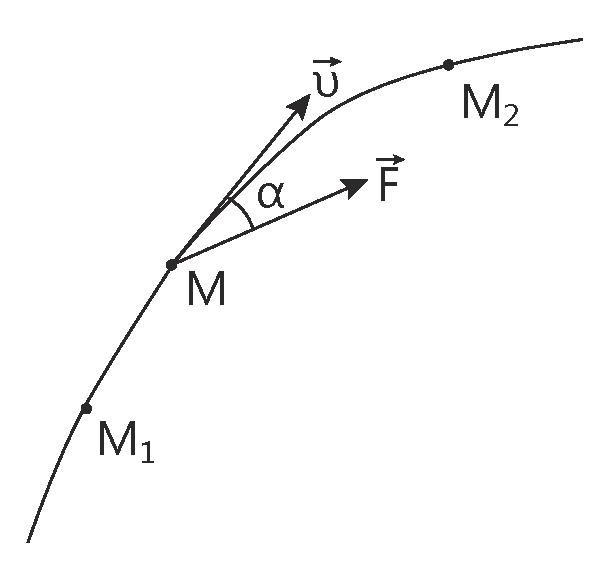
\includegraphics[width=.4\textwidth]{18_01} &
        Запишем основное уравнение динамики: \( \ds m\der{\vec{v}}{t} = \vec{F} \), где
        \( \vec{F} \) -- равнодействующая всех сил, приложенных к материальной точке.
        Помножим скалярно обе части на \( \d\vec{r} \):
        \[
            m\der{\vec{v}}{t}\cdot\d\vec{r} = \vec{F}\cdot\d\vec{r}.
        \]
        
        В правой части стоит элементарная работа \( \d A \) равнодействующей всех сил,
        приложенных к материальной точке; левую часть представим в следующем виде:
    \end{tabular}
\end{table}

\[
    m\der{\vec{v}}{t}\cdot\d\vec{r} = m\der{\vec{r}}{t}\cdot\d\vec{v} = m\vec{v}
    \cdot\d\vec{v} = \d\left(\frac{mv^2}{2}\right).
\]

Таким образом, имеем следующее равенство:
\( \ds \d\left(\frac{mv^2}{2}\right) = \d A\), то есть полный дифференциал
кинетической энергии материальной точки равен элементарной работе всех
действующих на эту точку сил. Проинтегрировав последнее выражение в пределах
от~\( M_1 \)~до~\( M_2 \), найдем окончательное уравнение для теоремы об изменении
кинетической энергии:
\[
    \frac{mv_2^2}{2} - \frac{mv_1^2}{2} = A.
\]

\section{Закон сохранения механической энергии}

Предположим, что все силы, действующие на материальную точку, потенциальны.
Тогда элементарная работа сил, приложенных к точке: \( \d A = -\d\varPi \) и
дифференциальная форма теоремы об изменении кинетической энергии примет вид:
\( \ds \d\left(\frac{mv^2}{2}\right) = -\d\varPi \). Интегрируя обе части этого
равенства, найдем: \( T + \varPi = h \), где \( h = \const \), то есть интеграл
энергии показывает, что при движении точки в потенциальном поле сил сумма
кинетической и потенциальной энергии (полная механическая энергия) есть величина
постоянная.

\newpage
